\documentclass[10pt,a4paper]{article}
\usepackage[T1]{fontenc}
\usepackage[utf8]{inputenc}
\usepackage[polish]{babel}
\usepackage{newtxtext,newtxmath}
\usepackage{microtype}
\usepackage[left=18mm,right=18mm,top=20mm,bottom=21mm,headheight=13pt,headsep=7mm,footskip=10mm]{geometry}
\usepackage{graphicx}
\usepackage[table]{xcolor}
\usepackage{array,booktabs,tabularx}
\usepackage{amsmath}
\usepackage{titlesec,fancyhdr,lastpage}
\usepackage{caption}
\usepackage{fvextra}
\usepackage{xurl}
\usepackage[unicode,hidelinks]{hyperref}

\definecolor{ink}{HTML}{172E3D}
\definecolor{accent}{HTML}{148A76}
\definecolor{muted}{HTML}{546B7B}
\definecolor{pale}{HTML}{EDF4F4}
\color{ink}
\hypersetup{
  pdftitle={PONG - przeciwnik uczący się grać. Sprawozdanie},
  pdfauthor={Artur Zamorowski, Kacper Wojtowicz, Rafał Wybraniec},
  pdflang={pl-PL}
}
\graphicspath{{../wyniki/}}
\setlength{\parindent}{0pt}
\setlength{\parskip}{5.5pt plus 1pt}
\linespread{1.06}
\setlength{\emergencystretch}{1.5em}
\clubpenalty=10000
\widowpenalty=10000
\raggedbottom
\titleformat{\section}{\sffamily\bfseries\LARGE\color{ink}}{\thesection.}{0.5em}{}
\titleformat{\subsection}{\sffamily\bfseries\normalsize\color{accent}}{}{0pt}{}
\titlespacing*{\section}{0pt}{0pt}{12pt}
\titlespacing*{\subsection}{0pt}{10pt}{4pt}
\captionsetup{font=small,labelfont=bf,labelsep=period,justification=raggedright,singlelinecheck=false,skip=6pt,hypcap=false}
\addto\captionspolish{\renewcommand{\figurename}{Rys.}}
\pagestyle{fancy}
\fancyhf{}
\fancyhead[L]{\sffamily\scriptsize\color{muted}Sztuczna inteligencja w grach i rozszerzonej rzeczywistości}
\fancyfoot[L]{\sffamily\scriptsize\color{muted}PONG / Projekt 1 / Zespół 1}
\fancyfoot[R]{\sffamily\scriptsize\color{muted}\thepage\ / \pageref*{LastPage}}
\renewcommand{\headrulewidth}{0pt}
\renewcommand{\footrulewidth}{0.3pt}
\fancypagestyle{cover}{\fancyhead{}}
\newcolumntype{L}[1]{>{\raggedright\arraybackslash}p{#1}}
\newcolumntype{Y}{>{\raggedright\arraybackslash}X}
\newenvironment{reporttable}[1]{%
  \par\smallskip\begingroup\small
  \renewcommand{\arraystretch}{1.23}%
  \setlength{\tabcolsep}{6pt}%
  \tabularx{\linewidth}{#1}\toprule\rowcolor{pale}%
}{\bottomrule\endtabularx\endgroup\par\smallskip}
\newcommand{\file}[1]{\path{#1}}
\newcommand{\scenario}[1]{\texttt{\detokenize{#1}}}
\newcommand{\clip}{\operatorname{clip}}
\DefineVerbatimEnvironment{commands}{Verbatim}{fontsize=\small,frame=single,rulecolor=\color{accent},framesep=7pt,breaklines=true}

\begin{document}
\thispagestyle{cover}
{\sffamily\bfseries\fontsize{34}{39}\selectfont PONG\par}
{\sffamily\bfseries\fontsize{23}{29}\selectfont Przeciwnik uczący się grać\par}
\vspace{5pt}
Projekt 1 / Zespół 1 / poniedziałek 8:00--10:15\\
Sztuczna inteligencja w grach i rozszerzonej rzeczywistości\\
Sprawozdanie, 15 listopada 2026 r.

\vspace{6pt}
Agent uczy się sterować prawą paletką na podstawie bieżącego stanu gry.
Porównano cztery tablice Q: siatki 50 i 100~px, każdą przy współczynniku
uczenia $\alpha=0{,}12$ i $\alpha=0{,}35$. Każdy model przeszedł
50\,000 epizodów. Ocenę końcową wykonano na 450 nowych serwisach dla
każdej polityki.

\begin{center}
  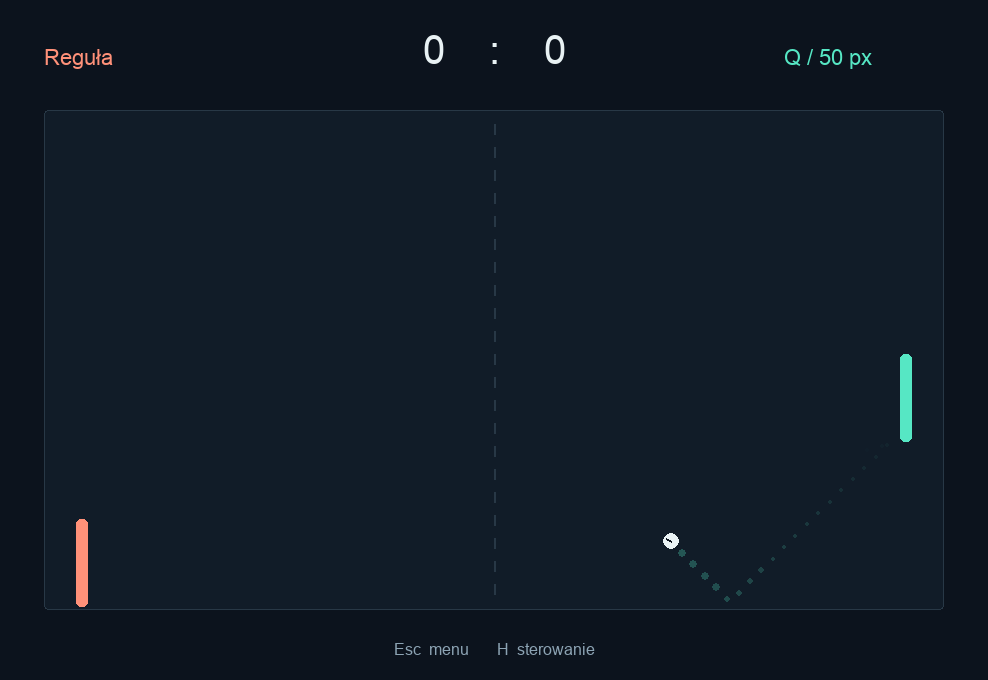
\includegraphics[width=0.93\linewidth]{gra.png}
  \captionof{figure}{Gra w trybie demonstracji. Wyuczony agent steruje prawą paletką.}
  \label{fig:gra}
\end{center}

\begin{reporttable}{L{37mm}Y}
  \textbf{Osoba} & \textbf{Odpowiedzialność} \\ \midrule
  Artur Zamorowski & Budowa i trenowanie modelu. \\
  Kacper Wojtowicz & Silnik gry, interfejs graficzny i przygotowanie prezentacji. \\
  Rafał Wybraniec & Sprawozdanie i dostosowywanie parametrów. \\
\end{reporttable}

\clearpage
\section{Zadanie i architektura}

Agent wybiera ruch w górę, postój albo ruch w dół, zapisane jako akcje
$-1$, $0$ i $+1$. Obserwacja zawiera pozycję i prędkość piłki oraz
pozycję i prędkość własnej paletki. Punkt kończy przejście piłki poza
boczną granicę boiska. W treningu i ocenie pojedynczy punkt ma limit
20~s czasu symulowanego. Mecz w interfejsie trwa do 7 zdobytych punktów.

\subsection*{Podział programu}
\begin{reporttable}{L{38mm}Y}
\textbf{Plik} & \textbf{Zadanie} \\ \midrule
\file{kod/main.py} & Wybór trybu, YAML, trening, ocena i zapis CSV. \\
\file{kod/pong/physics.py} & Stałe boiska, ruch, kolizje i punktacja. \\
\file{kod/pong/agents.py} & Stan siatkowy, tablica Q i reguła śledzenia piłki. \\
\file{kod/pong/gui.py} & Okno gry, klawiatura, menu i pauza. \\
\file{konfiguracja.yaml} & Modele, parametry uczenia, ziarna i liczba epizodów. \\
\end{reporttable}

Trening i gra korzystają z tej samej symulacji. Trening działa bez
rysowania i aktualizuje tablicę po każdej decyzji. Gra odczytuje gotowy
model. Fizyka pracuje ze stałym krokiem $1/120$~s, a agent podejmuje
30 decyzji na sekundę. Jedna akcja trwa cztery kroki fizyki.

Serwis losuje wysokość i kierunek lotu piłki oraz początkowe pozycje
paletek. Losowanie ma zapisane ziarno, więc ustawienia początkowe można
odtworzyć. Obie paletki mają te same ograniczenia ruchu.

\subsection*{Środowisko}
Program wymaga Pythona 3.11 lub nowszego. Pomiary wykonano w Pythonie
3.13.12. NumPy 2.3.5 przechowuje tablice Q, Pygame-ce 2.5.8 obsługuje
okno i klawiaturę, a PyYAML 6.0.3 odczytuje ustawienia. Sprawozdanie
jest składane z LaTeX-a. Wersje zależności zapisano w
\file{uruchomienie/wymagania.txt}.

Pliki modeli zawierają tablicę Q i metadane JSON: parametry fizyki,
rozmiar komórki, alfę, gammę, ziarno, budżet uczenia i wartości nagród.
\clearpage
\section{Fizyka rozgrywki}


Paletka przyspiesza i hamuje, więc agent musi rozpocząć ruch przed
nadejściem piłki. Miejsce trafienia i prędkość paletki zmieniają odbicie.
Ruch paletki nadaje też rotację, która zakrzywia dalszy tor lotu.

\begin{reporttable}{L{56mm}Y}
  \textbf{Parametr} & \textbf{Wartość} \\ \midrule
  Boisko / paletka / promień piłki & $900\times500$~px / $12\times88$~px / 8~px \\
  Prędkość / przyspieszenie paletki & 460~px/s / 3600~px/s$^2$, identyczne po obu stronach \\
  Szybkość piłki & 430~px/s na starcie, wzrost $\times1{,}06$ po odbiciu, limit 800~px/s \\
  Odbicie & Kąt zależny od miejsca trafienia, maks. 0,96~rad przed korektą ruchu \\
  Krok fizyki / decyzji & $1/120$~s / $1/30$~s \\
  Rotacja & Zakres $[-7,7]$, wykładniczy zanik z parametrem 0,55~s$^{-1}$ \\
\end{reporttable}

\subsection*{Przebieg pojedynczego kroku}
W każdym kroku symulator przesuwa paletki i ogranicza ich pozycje do
boiska. Potem oblicza wpływ rotacji na prędkość piłki, przesuwa ją
i rozpatruje kolizje. Jeśli piłka przekroczy powierzchnię odbicia,
zachowuje pozostałą część drogi po przeciwnej stronie. Piłka kontynuuje
ruch po odbiciu.

Niech $y_b$ i $y_p$ oznaczają wysokość piłki i środka paletki,
a $v_p$ prędkość paletki. Prędkości po odbiciu obliczamy ze wzorów:
\begin{align*}
  u &= \clip\!\left(\frac{y_b-y_p}{44},-1,1\right),\\
  V &= \min\!\left(800,\;1{,}06\sqrt{v_x^2+v_y^2}\right),\\
  v_y^{\mathrm{out}} &= \clip\!\left(V\sin(0{,}96u)+0{,}22v_p,\;-0{,}88V,\;0{,}88V\right),\\
  \left|v_x^{\mathrm{out}}\right| &= \sqrt{V^2-\left(v_y^{\mathrm{out}}\right)^2}.
\end{align*}

Rotacja wynosi $\omega=\clip(5v_p/460+2u,-7,7)$. W locie składnik
pionowy zmienia się o $0{,}13\omega v_x\,\mathrm{d}t$. Potem
normalizujemy wektor do poprzedniej szybkości. Rotacja zmienia kierunek
ruchu przy zachowaniu szybkości. Odbicie od poziomej ściany zmienia
znak i zmniejsza rotację współczynnikiem 0,8.

Sprawdzenie przecięcia czoła paletki wykrywa kontakt także wtedy, gdy
piłka przeskoczy tę płaszczyznę w jednym kroku. Pionowy zasięg kontaktu
obejmuje dodatkowo promień piłki, co upraszcza kolizje przy narożnikach.
Parametry fizyki dobrano do gry zręcznościowej.

\clearpage
\section{Stan agenta i uczenie}

Tablicowy Q-learning przypisuje każdemu stanowi trzy wartości, po jednej
dla każdej akcji. Wszystkie wartości zaczynają od zera.
\begin{equation*}
Q(s,a)\leftarrow Q(s,a)+\alpha\left[r+\gamma\max_{a'}Q(s',a')-Q(s,a)\right].
\end{equation*}
Po zdobyciu lub stracie punktu przyjmujemy $\max_{a'}Q(s',a')=0$.
Przy przerwaniu epizodu przez limit czasu aktualizacja nadal uwzględnia
wartość następnego stanu.

\subsection*{Stan}
Stan składa się z kolumny i wiersza piłki, wiersza paletki, znaku
$v_x$ oraz kategorii $v_y$ piłki i prędkości paletki. Pozycje dzielimy
przez rozmiar komórki i zaokrąglamy w dół. Granice kategorii pionowej
prędkości piłki wynoszą $-100$ i $100$~px/s, a dla paletki $-80$
i $80$~px/s.

\begin{reporttable}{L{35mm}Y L{25mm}}
\textbf{Siatka} & \textbf{Składowe liczby stanów} & \textbf{Stany} \\ \midrule
50~px & $18\cdot10\cdot10\cdot2\cdot3\cdot3$ & 32\,400 \\
100~px & $9\cdot5\cdot5\cdot2\cdot3\cdot3$ & 4050 \\
\end{reporttable}

Każdy wiersz tablicy Q ma trzy kolumny. Komórka $Q(s,a)$ przechowuje
oszacowaną wartość akcji $a$ w stanie $s$. Wybór zachłanny to akcja
z największą wartością w tym wierszu. Przy remisie wartości agent
preferuje postój.

\subsection*{Przejście i aktualizacja}
Następny stan $s'$ wyznacza symulator. Przez cztery kroki przesuwa
piłkę i paletki, rozpatruje odbicia, po czym nową obserwację funkcja
dyskretyzacji zamienia na numer wiersza. Rotacja piłki wpływa na tor
lotu, więc podobne stany siatkowe mogą prowadzić do różnych przejść.

Po decyzji aktualizowana jest komórka $Q(s,a)$ wykonanej akcji.
Składnik $\max_{a'}Q(s',a')$ odczytuje najlepszą z trzech wartości
następnego stanu. Informacja o nagrodzie przechodzi stopniowo do
wcześniejszych stanów w kolejnych epizodach. Aktualizacja odbywa się
również wtedy, gdy $s'=s$.

\subsection*{Nagrody i eksploracja}
Nagroda wynosi $+1$ za zdobyty punkt, $-1$ za stratę i $+0{,}2$
za odbicie własną paletką. Są to zdarzenia z wykonanej symulacji.
Współczynnik $\gamma=0{,}98$ określa wagę przyszłych nagród.

Epsilon maleje liniowo z 0,9 do 0,05 przez pierwsze 85\% epizodów.
W treningu agent z prawdopodobieństwem epsilon losuje akcję.
Podczas oceny epsilon wynosi zero.
\clearpage
\section{Protokół eksperymentów}

Porównanie obejmuje dwa rozmiary siatki i dwie wartości alfy. Każda
kombinacja rozpoczyna uczenie od zerowej tablicy. Ziarno treningu
wynosi 7. Wspólne ziarno zapewnia takie same serwisy w kolejnych
przebiegach. Dalszy lot zależy od wybranych akcji.

\begin{reporttable}{Yrr}
\textbf{Model} & \textbf{Komórka [px]} & $\boldsymbol{\alpha}$ \\ \midrule
\scenario{grid50_a012} & 50 & 0,12 \\
\scenario{grid50_a035} & 50 & 0,35 \\
\scenario{grid100_a012} & 100 & 0,12 \\
\scenario{grid100_a035} & 100 & 0,35 \\
\end{reporttable}

\begin{reporttable}{L{40mm}Y}
\textbf{Ustawienie} & \textbf{Wartość} \\ \midrule
Budżet & 50\,000 epizodów na model, łącznie 200\,000. \\
Punkty kontrolne & 0, 1000, 5000, 10\,000, 20\,000, 50\,000 epizodów. \\
Walidacja & 180 punktów, ziarna 1000000--1000179. \\
Ocena końcowa & 450 punktów na politykę, ziarna 2000000--2000449. \\
Przeciwnik & Reguła śledząca aktualną wysokość piłki, martwa strefa 12~px. \\
Częstość decyzji & 30~Hz po obu stronach. \\
Współbieżność & Dwa procesy treningowe. \\
\end{reporttable}

Reguła przesuwa paletkę w stronę bieżącej wysokości piłki. Przy różnicy
mniejszej niż 12~px wybiera postój. Korzysta z tej samej prędkości
maksymalnej i przyspieszenia co agent. Oceniono także regułę sterującą
prawą paletką przeciw takiemu samemu przeciwnikowi po lewej.

Mierzymy udział wygranych punktów, straty, remisy po limicie 20~s,
liczbę odbić obu paletek oraz czas trwania punktu. Cztery modele
oraz reguła dają łącznie 2250 punktów oceny końcowej.

Walidacja i ocena korzystają z osobnych ziaren. Wyniki dotyczą
pojedynczego ziarna uczenia dla każdej kombinacji parametrów.
Kolejne ziarna pozwoliłyby sprawdzić powtarzalność uzyskanej kolejności
modeli. Do gry domyślnie wybrano \scenario{grid50_a012}.
\clearpage
\section{Wyniki uczenia}

\begin{center}
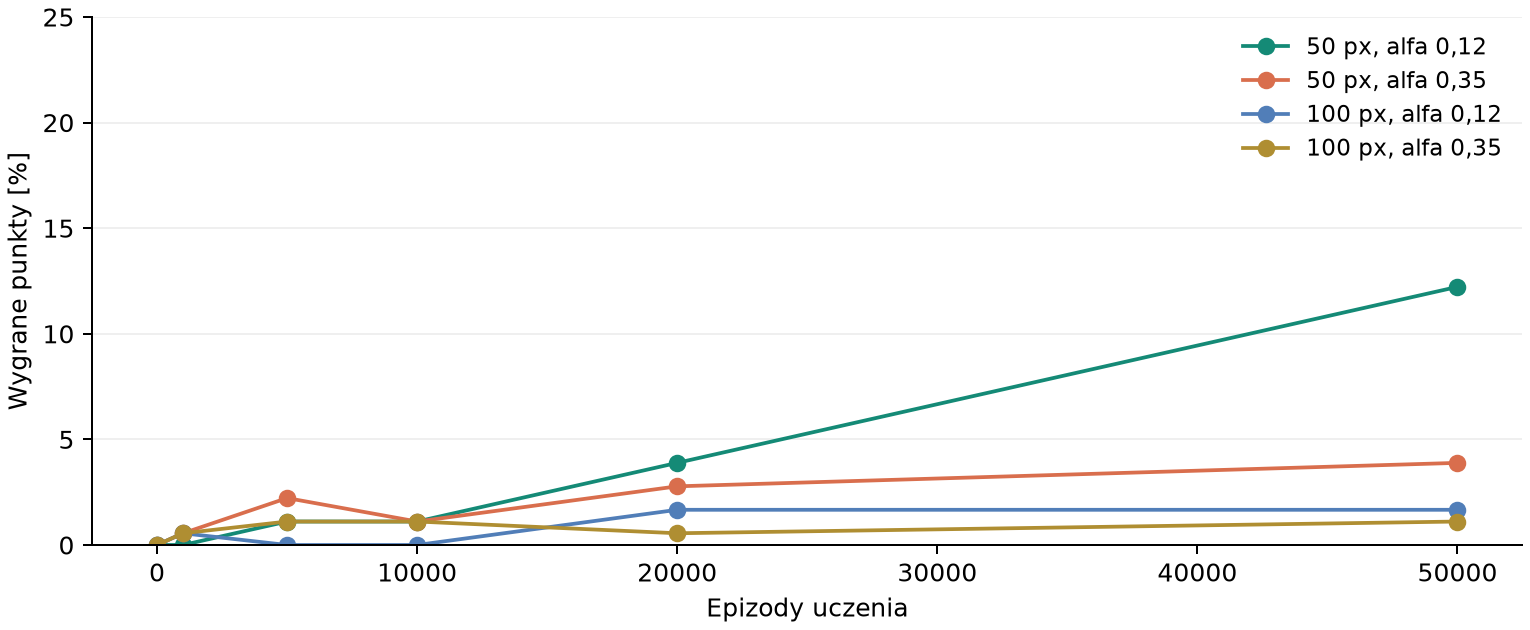
\includegraphics[width=\linewidth]{uczenie.png}
\captionof{figure}{Ocena w punktach kontrolnych. Każdy punkt wykresu obejmuje 180 serwisów.}
\end{center}

\begin{reporttable}{Yrrrr}
\textbf{Polityka} & \textbf{Wygrane} & \textbf{Straty} & \textbf{Remisy} & \textbf{Odbicia} \\ \midrule
50 px, $\alpha=$ 0,12 & 66 (14,7\%) & 349 & 35 & 6,45 \\
50 px, $\alpha=$ 0,35 & 18 (4,0\%) & 425 & 7 & 3,97 \\
100 px, $\alpha=$ 0,12 & 15 (3,3\%) & 432 & 3 & 3,61 \\
100 px, $\alpha=$ 0,35 & 6 (1,3\%) & 443 & 1 & 2,49 \\
Reguła & 77 (17,1\%) & 155 & 218 & 12,43 \\
\end{reporttable}

Spośród tablic Q najwyższy wynik oceny końcowej uzyskał model 50 px, alfa 0,12: 14,7\% wygranych punktów. Wygrał 66, przegrał 349, a 35 wymian zakończył limitem czasu. Średnia długość punktu wyniosła 11,84~s, a liczba odbić 6,45.

Krzywe pokazują wynik zamrożonej polityki w kolejnych punktach
kontrolnych. Epsilon używany w treningu wpływa na zbierane doświadczenia.
Wartości na wykresie pochodzą z osobnej gry z epsilon równym zero.
\clearpage
\section{Porównanie modeli}

\begin{center}
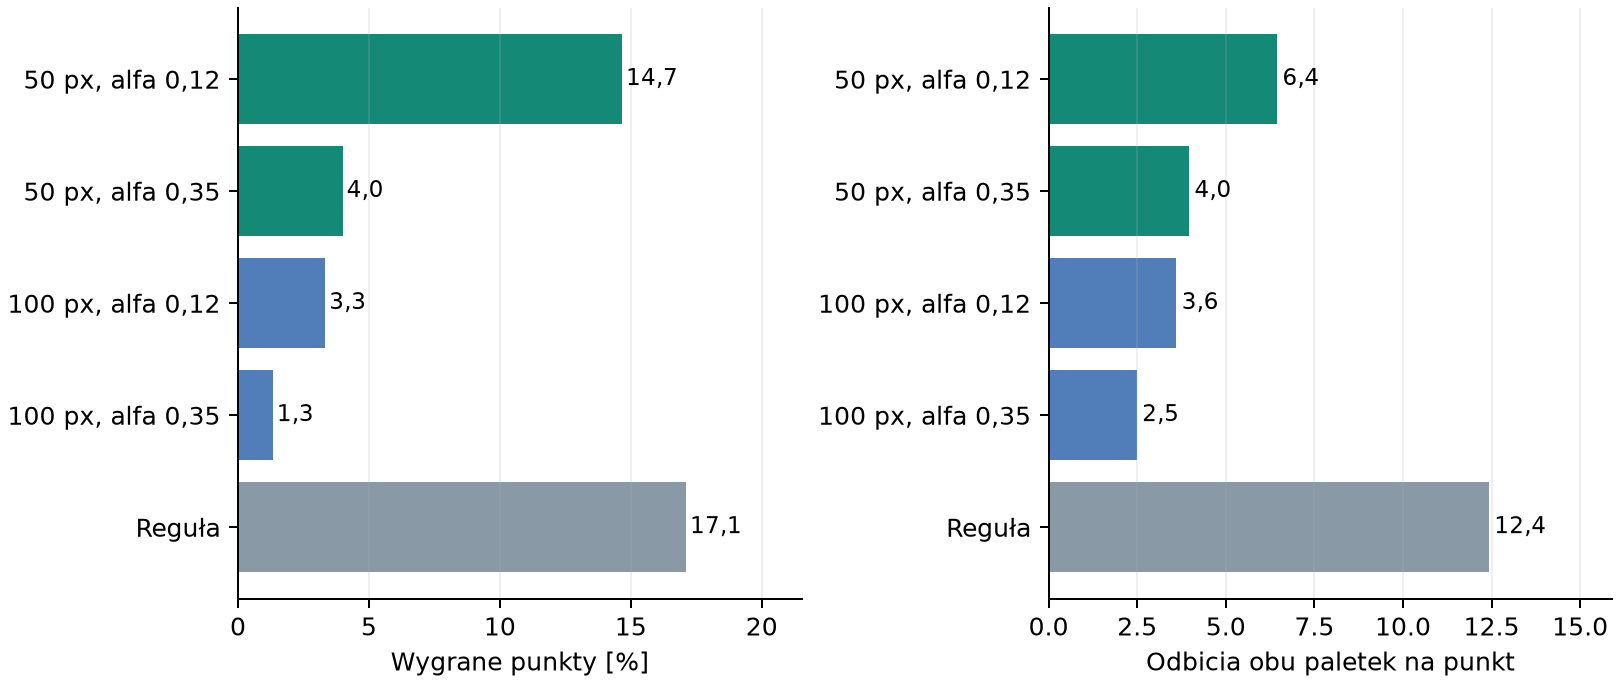
\includegraphics[width=\linewidth]{porownanie.png}
\captionof{figure}{Ocena na wspólnych 450 serwisach: wygrane punkty i długość wymian.}
\end{center}

Dla siatki 50~px udział wygranych wyniósł 14,7\% przy $\alpha=0{,}12$ oraz 4,0\% przy $\alpha=0{,}35$. Średnia liczba odbić wyniosła odpowiednio 6,45 i 3,97.

Dla siatki 100~px udział wygranych wyniósł 3,3\% przy $\alpha=0{,}12$ oraz 1,3\% przy $\alpha=0{,}35$. Średnia liczba odbić wyniosła odpowiednio 3,61 i 2,49.

Reguła odniesienia uzyskała 17,1\% wygranych, a średnia liczba odbić wyniosła 12,43. Wynik punktowy zależy również od sposobu odbicia: zachowanie
piłki przez dłuższy czas może doprowadzić do remisu po 20~s.

Siatka 50~px dokładniej rozróżnia pozycje i zawiera osiem razy więcej
stanów od siatki 100~px. Przy tym samym budżecie doświadczenia rozkładają
się na większą liczbę komórek. Alfa 0,35 nadaje większą wagę nowemu
przejściu niż alfa 0,12. Porównanie tych ustawień dotyczy zapisanych
przebiegów z ziarnem 7.
\clearpage
\section{Odtwarzalność i wnioski}

Parametry są w \file{konfiguracja.yaml}. Program ma trzy tryby:
\begin{commands}
python kod/main.py play
python kod/main.py train
python kod/main.py evaluate
\end{commands}
\texttt{play} wczytuje plik wskazany przez pole \texttt{model}.
Pole \texttt{demo: true} uruchamia pokaz reguła kontra agent.
\texttt{train} uczy wszystkie cztery modele i zapisuje ich ocenę.
\texttt{evaluate} ocenia gotowe tablice.

\file{wyniki/uczenie.csv} zawiera oceny w punktach kontrolnych.
\file{wyniki/ocena.csv} zawiera każdy punkt oceny końcowej, jego ziarno,
wynik, liczbę odbić i czas symulowany. Pliki NPZ przechowują tablicę Q
oraz parametry użyte podczas treningu.

\subsection*{Kompilacja sprawozdania}
Z katalogu \file{dokumentacja/} wykonaj:
\begin{commands}
latexmk -pdf -outdir=../tmp/latex sprawozdanie.tex
\end{commands}
Kompilacja wymaga TeX Live lub MiKTeX z \texttt{latexmk} i
\texttt{pdflatex}. Wykresy i zrzut są dołączone w \file{wyniki/}.

\subsection*{Ograniczenia}
Każdy wariant reprezentuje jeden trening. Podział prędkości na trzy
kategorie i dyskretyzacja pozycji łączą różne sytuacje w jeden stan.
Rotacja piłki wpływa na przejścia, a obserwacja agenta obejmuje sześć
bieżących wielkości. Dalsze badania powinny objąć kolejne ziarna i
większy budżet dla dokładniejszej siatki.

\subsection*{Wnioski}
Spośród modeli Q najwyższy odsetek wygranych uzyskał wariant 50 px, alfa 0,12. Reguła odniesienia osiągnęła wyższy wynik punktowy i dłuższe wymiany od każdego z czterech modeli. Wyniki zapisano wraz z długością wymian, co pozwala osobno ocenić
zdobywanie punktów i utrzymywanie piłki. Zapisane tablice umożliwiają
uruchomienie gry od razu po instalacji trzech bibliotek.

\end{document}
